% !TEX root = ../prospector.tex

\begin{figure}
\centering
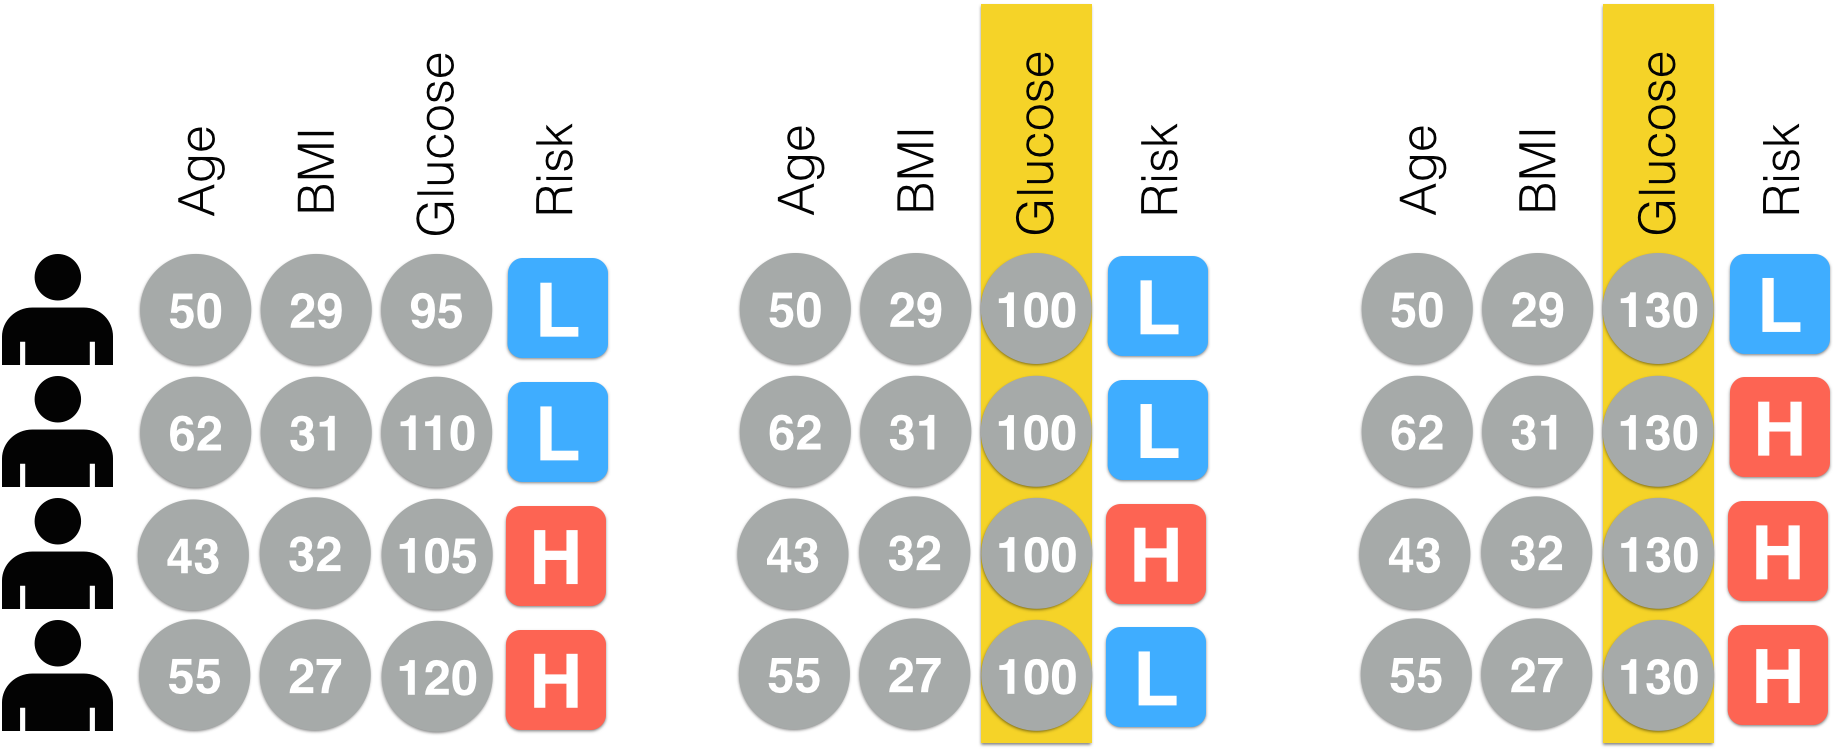
\includegraphics[width=0.90\linewidth]{prospector/partial-dependence-explanation} % 0.95
\caption{
An illustration of how partial dependence is computed for the feature ``Glucose".  On the left are four patients' original feature values.  In the middle, the ``Glucose" values are all changed to 100, and the corresponding predictions change.  Similarly, on the right, the ``Glucose" values are all changed to 130, and again the risks are different.  This demonstrates the impact of the ``Glucose'' feature on risk prediction.
% The plotted value in a Partial Dependence plot is the average of the
% ``Risk" probability values.
}
\label{figs:pdexplain}
\end{figure}